%==============================================================================
%  Oracle -- Distributed AI Infrastructure Platform
%  Technical Report (AI Academy project)
%
%  Build:  pdflatex oracle-technical-report.tex   (run twice for references)
%==============================================================================
\documentclass[11pt,a4paper]{article}

\usepackage[T1]{fontenc}
\usepackage[utf8]{inputenc}
\usepackage{lmodern}
\usepackage[margin=2.4cm,top=2.3cm,bottom=2.3cm]{geometry}
\usepackage{amsmath,amssymb}
\usepackage{graphicx}
\usepackage{booktabs}
\usepackage{array}
\usepackage{tabularx}
\usepackage{xcolor}
\usepackage{enumitem}
\usepackage{listings}
\usepackage{caption}
\usepackage{fancyhdr}
\usepackage{tikz}
\usetikzlibrary{arrows.meta,positioning,fit,backgrounds,calc,shapes.geometric}
\usepackage[hidelinks]{hyperref}

%------------------------------------------------------------------ style ----
\definecolor{oblue}{RGB}{23,74,124}
\definecolor{ogray}{RGB}{108,117,125}
\definecolor{ogreen}{RGB}{28,120,66}
\definecolor{oamber}{RGB}{176,116,10}
\definecolor{ored}{RGB}{160,40,40}
\definecolor{olight}{RGB}{238,243,248}

\captionsetup{font=small,labelfont={bf,color=oblue}}
\setlist{nosep,leftmargin=1.3em}
\setlength{\parskip}{0.35em}
\setlength{\parindent}{0pt}
\setlength{\emergencystretch}{3em}

\pagestyle{fancy}
\fancyhf{}
\fancyhead[L]{\footnotesize\color{ogray}Oracle -- Distributed AI Infrastructure Platform}
\fancyhead[R]{\footnotesize\color{ogray}\thepage}
\renewcommand{\headrulewidth}{0.4pt}

\lstdefinestyle{oracle}{
  basicstyle=\ttfamily\footnotesize,
  keywordstyle=\color{oblue}\bfseries,
  stringstyle=\color{ogreen},
  commentstyle=\color{ogray}\itshape,
  showstringspaces=false,
  breaklines=true,
  frame=single,
  rulecolor=\color{ogray!50},
  backgroundcolor=\color{olight},
  columns=fullflexible,
  xleftmargin=4pt, xrightmargin=4pt,
  aboveskip=6pt, belowskip=6pt
}
\lstset{style=oracle}

% implementation-status badges
\newcommand{\stImp}{\textcolor{ogreen}{\footnotesize\textsf{\textbf{IMPLEMENTED}}}}
\newcommand{\stPart}{\textcolor{oamber}{\footnotesize\textsf{\textbf{PARTIALLY IMPLEMENTED}}}}
\newcommand{\stPlan}{\textcolor{oblue}{\footnotesize\textsf{\textbf{PLANNED}}}}
\newcommand{\stFut}{\textcolor{ored}{\footnotesize\textsf{\textbf{FUTURE}}}}
\newcommand{\tbm}{\textcolor{ogray}{\emph{To be measured.}}}

% tikz shorthands
\tikzset{
  box/.style   ={rectangle, rounded corners=2pt, draw=oblue!70, fill=olight,
                 align=center, inner sep=4pt, font=\footnotesize},
  dark/.style  ={box, fill=oblue!15, draw=oblue, font=\footnotesize\bfseries},
  plain/.style ={rectangle, draw=ogray!70, fill=white, align=center,
                 inner sep=3.5pt, font=\scriptsize},
  ar/.style    ={-{Stealth[length=2mm]}, draw=oblue!80, thick},
  arg/.style   ={-{Stealth[length=2mm]}, draw=ogray, thin},
  lbl/.style   ={font=\scriptsize\itshape, text=ogray}
}

\begin{document}

%============================================================== COVER PAGE ====
\begin{titlepage}
\centering
\vspace*{1.6cm}

{\Huge\bfseries\color{oblue} ORACLE\par}
\vspace{0.5em}
{\LARGE Distributed AI Infrastructure Platform\par}
\vspace{0.9em}
{\large\itshape Turning several physically connected computers into one\\ AI inference cluster\par}

\vspace{1.4cm}
\rule{0.75\textwidth}{0.8pt}
\vspace{1.0cm}

{\large\bfseries Technical Report\par}
\vspace{0.3em}
{\normalsize Version 0.1 --- Engineering prototype\par}

\vspace{1.6cm}

\begin{tabular}{r@{\hspace{1.2em}}l}
\textbf{Project} & Oracle -- Distributed AI Infrastructure Platform \\[0.35em]
\textbf{Repository} & \url{https://github.com/Amouriii/Oracle} \\[0.35em]
\textbf{Course} & AI Academy --- Capstone Project \\[0.35em]
\textbf{Duration} & Approximately one week of development \\[0.35em]
\textbf{Date} & \today \\
\end{tabular}

\vspace{1.4cm}
{\large\bfseries Team Members\par}
\vspace{0.6em}
\begin{tabular}{ll}
Ahmed Abdelfattah & \textit{Project lead --- engine, transport, orchestration} \\[0.25em]
% ---------------------------------------------------------------------------
% TODO: replace the placeholder rows below with the remaining team members.
% ---------------------------------------------------------------------------
\rule{4.5cm}{0.4pt} & \rule{5.5cm}{0.4pt} \\[0.25em]
\rule{4.5cm}{0.4pt} & \rule{5.5cm}{0.4pt} \\[0.25em]
\rule{4.5cm}{0.4pt} & \rule{5.5cm}{0.4pt} \\
\end{tabular}

\vfill
{\footnotesize\color{ogray}
This report describes an academic engineering prototype. Implementation status is
stated per component and is derived from the project repository. Oracle is
\textbf{not} a production system, and no performance numbers are claimed unless
they have been measured.\par}
\end{titlepage}

%================================================================= ABSTRACT ===
\section*{Abstract}
\addcontentsline{toc}{section}{Abstract}

Modern large language models routinely require more memory than a single
ordinary workstation can provide, which places them out of reach for teams that
own several medium-sized machines but no large accelerator. Oracle addresses
this gap by treating a small group of physically connected computers as a single
AI inference platform. A model is split layer-by-layer across the machines; each
machine holds only its own shard of weights and its own slice of the attention
key/value cache, and passes intermediate activations to the next machine over a
high-speed local link using a compact binary tensor protocol. A master node owns
the public interface: it exposes an OpenAI-compatible HTTP API, plans how the
model is distributed across the cluster from the model's own metadata and each
node's memory budget, tracks node health through UDP heartbeats, and refuses work
when the cluster cannot safely serve it. The prototype implements the
distributed dataflow, the sharding planner, the health layer and the API surface;
concurrent multi-request serving, weight-level model execution and the security
layer are specified in this report and are partially implemented or planned.
Oracle's expected impact is to make large-model inference reachable on
commodity hardware that organisations already own.

%============================================================= INTRODUCTION ===
\section{Introduction}

The practical cost of running a large AI model is dominated by a single
constraint: the model's parameters, its activations, and its attention cache
must all be resident in memory at the same time. A 70-billion-parameter model
quantised to roughly four bits per weight occupies on the order of 35--40~GiB of
weights alone, before any per-request key/value (KV) cache is allocated. A
machine that cannot hold that working set either cannot run the model at all, or
falls back to swapping weights from storage on every token, which slows
generation by orders of magnitude.

Beyond memory, serving a model imposes three further demands:

\begin{itemize}
  \item \textbf{Compute.} Each generated token requires a full forward pass over
        every layer. Matrix multiplication throughput, not clock speed, sets the
        token rate.
  \item \textbf{Storage.} Model files are tens of gigabytes; loading them is a
        measurable part of start-up time and must be planned, not improvised.
  \item \textbf{Networking.} As soon as a model is split across machines,
        intermediate activations must cross the network on every token. The link
        between machines becomes part of the inference path, and its latency is
        paid once per hop per token.
\end{itemize}

Relying on a single computer therefore creates a hard ceiling. Buying a larger
machine or renting cloud accelerators solves the problem with money rather than
with engineering, and neither option is available to every student, laboratory
or small organisation. What such groups often \emph{do} have is several ordinary
computers.

\textbf{Oracle} is a distributed AI inference platform that combines those
machines. Computers are connected over a dedicated high-speed link --- in the
reference deployment, a Thunderbolt~3 bridge --- and cooperate to serve a model
that no single member could hold. One machine acts as the \emph{master}: it
terminates client requests, decides how the model is laid out across the
cluster, monitors the other machines, and returns generated tokens. The others
act as \emph{workers}: each owns a contiguous range of model layers and executes
only that range. From the outside, the whole cluster looks like one endpoint
speaking the OpenAI chat-completions protocol.

This report describes Oracle's design, states precisely which parts of that
design are implemented in the current prototype, and sets out what remains.

%======================================================= PROBLEM & OBJECTIVES =
\section{Problem Statement and Objectives}

\subsection{Problem statement}

\emph{Given a small number of ordinary computers connected by a fast local link,
serve a large AI model that exceeds the memory of any single machine, expose it
through a standard API, keep serving while machines come and go, and do so
without assuming specialised datacentre hardware.}

Three sub-problems follow directly. First, \textbf{placement}: the model must be
divided so that every machine's share fits inside its declared memory budget,
including the KV cache that grows with sequence length. Second,
\textbf{coordination}: the machines must exchange activations for every token
with low enough overhead that the network does not dominate the token rate.
Third, \textbf{trust and liveness}: a cluster with one unresponsive machine must
detect that fact and fail loudly, rather than blocking indefinitely on a machine
that will never answer.

\subsection{Objectives}

\begin{table}[h]
\centering
\caption{Project objectives and how each is addressed in the current prototype.}
\label{tab:objectives}
\footnotesize
\begin{tabularx}{\textwidth}{@{}l X l@{}}
\toprule
\textbf{Objective} & \textbf{Meaning in Oracle} & \textbf{Status} \\
\midrule
Distributed AI inference & Split one forward pass across several machines & \stImp \\
Large-model support & Layer sharding sized against per-node RAM budgets & \stImp \\
Multi-request serving & Serve several client requests at once & \stPart \\
Parallel execution & Overlap work instead of a strict serial pipeline & \stPlan \\
Intelligent orchestration & Place layers from model metadata + node resources & \stPart \\
Model recognition & Read model architecture and size from the model file & \stImp \\
Heartbeat / monitoring & Detect unresponsive nodes and act on it & \stImp \\
Security & Authenticate clients and nodes, bound resource usage & \stPlan \\
Deployment & Reproducible build and native cluster binaries & \stImp \\
OpenAI-compatible API & Existing clients work unchanged & \stImp \\
\bottomrule
\end{tabularx}
\end{table}

Status labels are used consistently throughout this report:
\stImp{} means the behaviour exists in the repository and is exercised by tests
or scripts; \stPart{} means the mechanism exists but is incomplete or
placeholder in an important respect; \stPlan{} means it is designed and
specified here but not yet coded; \stFut{} means it is a longer-term direction.

%============================================================== ARCHITECTURE ==
\section{Oracle System Architecture}

Oracle is a master/worker system. Exactly one node carries the \texttt{master}
role and owns everything client-facing and cluster-wide; every other node is a
worker that executes a slice of the model and nothing else. All nodes run the
same engine library and differ only in configuration and entry-point binary.

\begin{figure}[h]
\centering
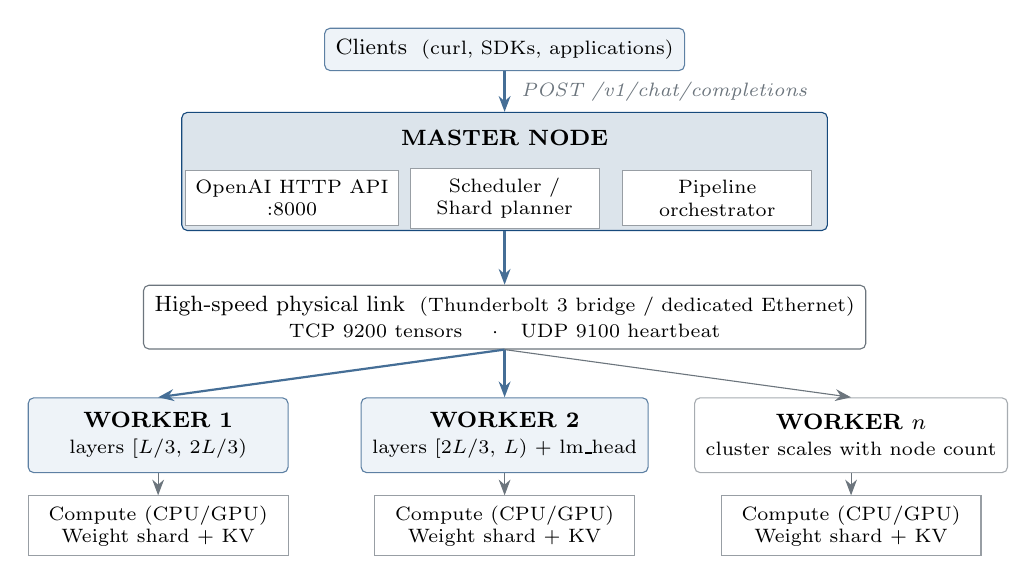
\begin{tikzpicture}

\node[box, minimum width=3.6cm] (client) at (0,1.55)
  {Clients \;\scriptsize(curl, SDKs, applications)};

\node[dark, minimum width=8.2cm, minimum height=1.5cm] (master) at (0,0) {};
\node[font=\footnotesize\bfseries, anchor=north] at ([yshift=-3pt]master.north) {MASTER NODE};
\node[plain, minimum width=2.4cm] (api)   at (-2.7,-0.34) {OpenAI HTTP API\\\scriptsize:8000};
\node[plain, minimum width=2.4cm] (sched) at ( 0.0,-0.34) {Scheduler /\\Shard planner};
\node[plain, minimum width=2.4cm] (orch)  at ( 2.7,-0.34) {Pipeline\\orchestrator};
\draw[ar] (client) -- node[lbl,right]{\;POST /v1/chat/completions} (master);

\node[box, minimum width=8.2cm, fill=white, draw=ogray] (link) at (0,-1.85)
  {High-speed physical link \;\scriptsize(Thunderbolt~3 bridge / dedicated Ethernet)\\
   \scriptsize TCP 9200 tensors \quad$\cdot$\quad UDP 9100 heartbeat};
\draw[ar] (master) -- (link);

\node[box, minimum width=3.3cm, minimum height=0.95cm] (w1) at (-4.4,-3.35)
  {\textbf{WORKER 1}\\\scriptsize layers $[L/3,\,2L/3)$};
\node[box, minimum width=3.3cm, minimum height=0.95cm] (w2) at ( 0.0,-3.35)
  {\textbf{WORKER 2}\\\scriptsize layers $[2L/3,\,L)$ + lm\_head};
\node[box, minimum width=3.3cm, minimum height=0.95cm, draw=ogray!60, fill=white]
  (w3) at ( 4.4,-3.35)
  {\textbf{WORKER $n$}\\\scriptsize cluster scales with node count};

\draw[ar] (link.south) -- (w1.north);
\draw[ar] (link.south) -- (w2.north);
\draw[arg] (link.south) -- (w3.north);

\node[plain, minimum width=3.3cm] (c1) at (-4.4,-4.5) {Compute (CPU/GPU)\\Weight shard + KV};
\node[plain, minimum width=3.3cm] (c2) at ( 0.0,-4.5) {Compute (CPU/GPU)\\Weight shard + KV};
\node[plain, minimum width=3.3cm] (c3) at ( 4.4,-4.5) {Compute (CPU/GPU)\\Weight shard + KV};
\draw[arg] (w1) -- (c1);
\draw[arg] (w2) -- (c2);
\draw[arg] (w3) -- (c3);
\end{tikzpicture}
\caption{Oracle cluster architecture. The master owns the API, placement and
orchestration; workers own layer shards and local KV state. Activations travel
master $\rightarrow$ worker $\rightarrow \dots \rightarrow$ master once per
generated token.}
\label{fig:arch}
\end{figure}

\begin{table}[h]
\centering
\caption{System components and implementation status.}
\label{tab:components}
\footnotesize
\begin{tabularx}{\textwidth}{@{}l l X l@{}}
\toprule
\textbf{Component} & \textbf{Module} & \textbf{Responsibility} & \textbf{Status} \\
\midrule
Tensor transport & \texttt{tb3-transport} & Packed binary tensor frames over TCP,
  shared-memory ring for the local hop, UDP heartbeat socket & \stImp \\
Shard manager & \texttt{mem-shard-manager} & Layer assignment, KV cache planning,
  memory-budget feasibility, host memory-pressure sampling & \stImp \\
Orchestrator & \texttt{orchestrator-core} & Pipeline DAG, token loop, heartbeat
  bookkeeping, OpenAI HTTP server & \stImp \\
Node runners & \texttt{metal-cpu-runner} & Pluggable compute back ends
  (Accelerate BLAS, Metal GEMM, llama.cpp/GGUF) & \stPart \\
Master binary & \texttt{oracle-engine-master} & Entry point: config, API, cluster
  bring-up & \stImp \\
Worker binary & \texttt{oracle-engine-worker} & Entry point: receive, compute,
  forward & \stImp \\
Network bench & \texttt{oracle-engine-bench-net} & Link throughput and
  round-trip measurement tool & \stImp \\
Dashboard UI & --- & Cluster health and utilisation visualisation & \stPlan \\
Security layer & --- & Authentication, rate limiting, node identity & \stPlan \\
\bottomrule
\end{tabularx}
\end{table}

\textbf{Master.} Loads the cluster description, asks the shard manager for a
placement, builds the execution graph, opens the tensor transport and the
heartbeat socket, and then serves HTTP. It performs embedding and the first
layer range itself, so the master is a compute participant, not only a
coordinator.

\textbf{Workers.} Each worker connects to its predecessor in the chain, blocks on
the transport, runs its own layer range over each activation tensor it receives,
and forwards the result to its successor. The final worker additionally applies
the output projection (\texttt{lm\_head}) and sends logits back to the master.

\textbf{Transport.} A single packed 76-byte header (\texttt{TensorHeader},
magic \texttt{ORCL}) followed by a raw payload. There is no JSON or protobuf on
the hot path; header and body are written together with \texttt{writev} and the
payload carries a CRC32. For two processes on the same machine, a lock-free
single-producer/single-consumer shared-memory ring replaces the socket.

%================================================= DISTRIBUTED AI INFERENCE ===
\section{Distributed AI Inference}

\subsection{How a model is split}

Oracle divides a model along its \emph{layer} axis. Given a model with $L$
transformer blocks and $n$ nodes, the shard manager assigns each node a
contiguous range so that the ranges tile $[0,L)$ exactly. For a 70B-class model
with $L=80$ and three nodes, each node owns roughly 26--27 consecutive layers
and about one third of the weights.

\begin{figure}[h]
\centering
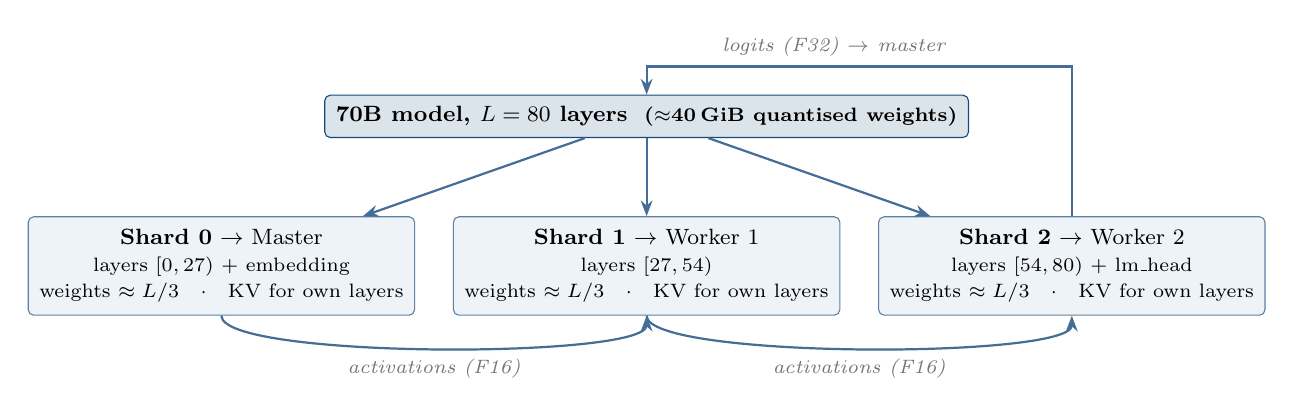
\begin{tikzpicture}
\node[dark, minimum width=5.4cm] (model) at (0,1.9)
  {70B model, $L=80$ layers \;\scriptsize($\approx$40\,GiB quantised weights)};

\node[box, minimum width=4.7cm, minimum height=1.25cm] (s1) at (-5.4,0)
  {\textbf{Shard 0} $\rightarrow$ Master\\\scriptsize layers $[0,27)$ + embedding\\
   \scriptsize weights $\approx L/3$ \; $\cdot$ \; KV for own layers};
\node[box, minimum width=4.7cm, minimum height=1.25cm] (s2) at ( 0.0,0)
  {\textbf{Shard 1} $\rightarrow$ Worker 1\\\scriptsize layers $[27,54)$\\
   \scriptsize weights $\approx L/3$ \; $\cdot$ \; KV for own layers};
\node[box, minimum width=4.7cm, minimum height=1.25cm] (s3) at ( 5.4,0)
  {\textbf{Shard 2} $\rightarrow$ Worker 2\\\scriptsize layers $[54,80)$ + lm\_head\\
   \scriptsize weights $\approx L/3$ \; $\cdot$ \; KV for own layers};

\draw[ar] (model) -- (s1);
\draw[ar] (model) -- (s2);
\draw[ar] (model) -- (s3);

\draw[ar] (s1.south) .. controls +(0,-0.55) and +(0,-0.55) ..
  node[lbl,below]{activations (F16)} (s2.south);
\draw[ar] (s2.south) .. controls +(0,-0.55) and +(0,-0.55) ..
  node[lbl,below]{activations (F16)} (s3.south);
\draw[ar] (s3.north) -- ++(0,1.9)
  -| node[lbl,above,pos=0.28]{logits (F32) $\rightarrow$ master} (model.north);
\end{tikzpicture}
\caption{Layer-wise model sharding. Each node stores only its own weight shard
and the KV cache for its own layers; only a single hidden-state vector crosses
the link per hop per token.}
\label{fig:shard}
\end{figure}

\textbf{Distributed memory.} Two distinct memory pools are planned per node:
the weight shard (proportional to the node's layer count) and the KV cache. The
KV cache is sized from the model's own geometry --- for each local layer,
$2 \times n_{kv} \times d_{head} \times \texttt{max\_seq}$ elements for keys and
values --- and stays permanently on the node that owns those layers. It is never
transferred, which is precisely why per-token network traffic stays small.

\textbf{Activation transfer.} What crosses the link is one hidden-state vector
per hop per token. For a hidden dimension of 8192 in half precision, that is
about 16~KiB. On a Thunderbolt-3-class link this is a small payload, and the cost
per hop is dominated by round-trip latency rather than bandwidth.

\textbf{Worker computation and result propagation.} A worker receives the tensor,
validates the magic number and CRC, runs its layer range while updating its local
KV cache, and forwards the result. The last node in the chain produces the
vocabulary-sized logits vector and sends it to the master, which samples the next
token, embeds it, and starts the next round. Generation stops at the end-of-text
token or when \texttt{max\_tokens} is reached.

\subsection{Which kinds of parallelism are actually used}

The word ``parallelism'' covers several different techniques, and it is important
not to conflate them.

\begin{table}[h]
\centering
\caption{Forms of parallelism: definition and status in Oracle.}
\label{tab:parallel}
\footnotesize
\begin{tabularx}{\textwidth}{@{}l X l@{}}
\toprule
\textbf{Form} & \textbf{What it means} & \textbf{Status} \\
\midrule
\textbf{Pipeline parallelism} &
  Consecutive layer ranges live on different machines; a token's forward pass
  visits them in sequence. This is Oracle's core mechanism. & \stImp \\
\textbf{Model (tensor) parallelism} &
  A \emph{single} layer's matrices are split across machines, which then perform
  a collective reduction. Oracle does not do this; a layer always executes
  entirely on one node. & \stFut \\
\textbf{Request-level parallelism} &
  Several independent client requests progress at the same time. The HTTP server
  is multi-threaded and the wire protocol carries a per-request sequence
  identifier, but the orchestrator currently shares one KV cache and one pipeline
  ring, so requests are not yet isolated from each other. & \stPart \\
\textbf{Pipeline overlap} &
  While node~2 works on token $t$, node~1 already starts token $t{+}1$, so nodes
  are not idle. Not yet implemented: the current loop is strictly sequential per
  token. & \stPlan \\
\bottomrule
\end{tabularx}
\end{table}

\subsection{Honest note on model execution}

The distributed dataflow --- sharding, transport, pipeline traversal, KV
planning, sampling and streaming --- is implemented and testable end to end.
The \emph{numerics} inside a layer are not yet those of a real transformer: the
Accelerate back end currently loads identity matrices as placeholder layer
weights, and the llama.cpp back end reads real GGUF metadata but delegates the
forward pass to the same placeholder path unless the library is linked at build
time. In other words, Oracle today moves the right tensors, of the right shapes,
along the right path, at the right time, but does not yet produce meaningful text.
Wiring real GGUF weight execution into the runner interface is the single most
important next step and is listed as such in Section~\ref{sec:future}.

%======================================================== SCALE: MODELS/REQS ==
\section{Handling Large Models and Many Requests}

Oracle scales along two independent axes, and the two must not be confused: one
is about \emph{how big} a model can be, the other about \emph{how many} clients
can be served.

\subsection{Dimension A --- model scalability}

Adding a node adds its RAM budget to the cluster's pooled capacity. With $n$
nodes each declaring a budget $B_i$, the shard manager accepts a placement only
if, for every node, the weights of its assigned layers plus that node's KV cache
fit within $B_i$. This check is performed before any weights are loaded, so an
infeasible cluster is rejected at planning time with a specific reason rather
than failing later with an out-of-memory error. A companion pressure monitor
samples real host memory and refuses allocations that would overcommit the
machine even when the configured budget would allow them.

The consequence is straightforward: a model that does not fit on one machine may
fit on three, and Oracle can tell you \emph{before} you try.

\subsection{Dimension B --- request scalability}

\begin{figure}[h]
\centering
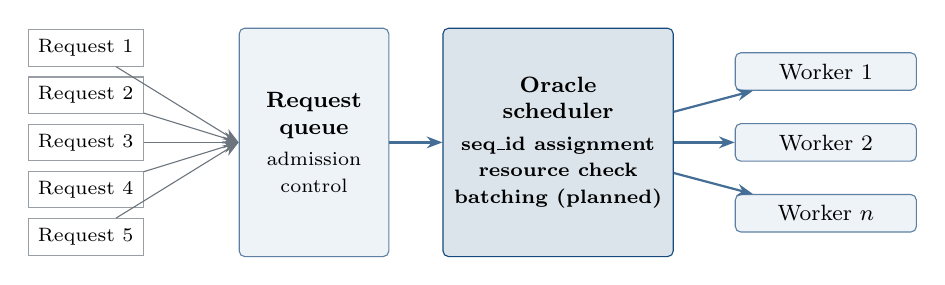
\begin{tikzpicture}[node distance=4mm]
\node[plain] (r1) at (0, 1.35) {Request 1};
\node[plain] (r2) at (0, 0.75) {Request 2};
\node[plain] (r3) at (0, 0.15) {Request 3};
\node[plain] (r4) at (0,-0.45) {Request 4};
\node[plain] (r5) at (0,-1.05) {Request 5};

\node[box, minimum height=2.9cm, minimum width=1.9cm] (q) at (2.9,0.15)
  {\textbf{Request}\\\textbf{queue}\\[2pt]\scriptsize admission\\\scriptsize control};
\foreach \r in {r1,r2,r3,r4,r5}{\draw[arg] (\r) -- (q.west);}

\node[dark, minimum height=2.9cm, minimum width=2.3cm] (s) at (6.0,0.15)
  {\textbf{Oracle}\\\textbf{scheduler}\\[2pt]\scriptsize seq\_id assignment\\
   \scriptsize resource check\\\scriptsize batching (planned)};
\draw[ar] (q) -- (s);

\node[box, minimum width=2.3cm] (wa) at (9.4, 1.05) {Worker 1};
\node[box, minimum width=2.3cm] (wb) at (9.4, 0.15) {Worker 2};
\node[box, minimum width=2.3cm] (wc) at (9.4,-0.75) {Worker $n$};
\foreach \w in {wa,wb,wc}{\draw[ar] (s) -- (\w);}
\end{tikzpicture}
\caption{Multi-request scheduling model. Requests are admitted, given a sequence
identifier, and dispatched onto the shared worker pipeline. The queue and
scheduler stages are the target design; the current build exposes a
thread-pooled HTTP front end over a single shared pipeline.}
\label{fig:sched}
\end{figure}

The intended behaviour, and its present state, are as follows.

\begin{itemize}
  \item \textbf{Request queue.} Incoming requests are accepted into a bounded
        queue rather than each spawning unbounded work. \stPlan
  \item \textbf{Scheduling.} Each request receives a unique sequence identifier
        that travels inside every tensor header, so any node can attribute an
        activation to the request it belongs to. The identifier and its wire
        field exist today. \stPart
  \item \textbf{Concurrency.} The HTTP layer already dispatches requests onto a
        thread pool. What is missing is per-request isolation inside the engine:
        the KV cache and the pipeline ring are currently shared, so concurrent
        requests would interfere. Giving each sequence its own KV slice and its
        own in-flight slot on the ring is the concrete work item. \stPart
  \item \textbf{Batching.} Grouping the decode steps of several sequences into
        one matrix multiplication is the standard way to raise throughput, and
        the transport already tolerates variable payload sizes. Not implemented.
        \stPlan
  \item \textbf{Resource allocation.} KV memory per sequence is computed from
        model geometry, so the maximum number of concurrent sequences a node can
        hold is a derivable quantity rather than a guess. \stImp{} (planner)
  \item \textbf{Avoiding unnecessary serialisation.} A pipeline whose stages run
        strictly one after another leaves $n{-}1$ of $n$ nodes idle at any
        instant. Overlapping consecutive tokens or sequences across stages is
        what turns the chain into a true pipeline. \stPlan
\end{itemize}

No claim is made about how many simultaneous requests Oracle can serve. That
number depends on model geometry, sequence length and node memory, and it has
not been measured; see Section~\ref{sec:eval}.

%============================================================== ORCHESTRATOR ==
\section{AI Orchestrator}

The orchestrator is the part of the master that turns a description of the
cluster and a description of the model into an executable plan, and then keeps
that plan honest at run time.

\begin{figure}[h]
\centering
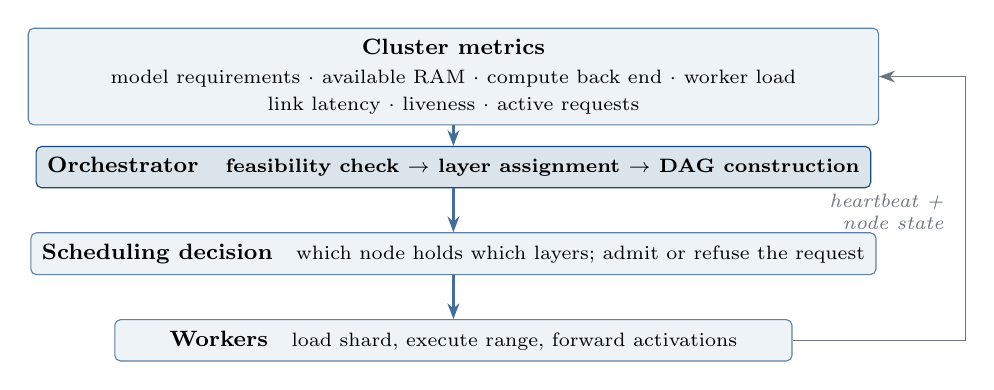
\begin{tikzpicture}[node distance=7mm]
\node[box, minimum width=10.8cm] (metrics) at (0,0)
  {\textbf{Cluster metrics}\\[1pt]
   \scriptsize model requirements $\cdot$ available RAM $\cdot$ compute back end
   $\cdot$ worker load\\
   \scriptsize link latency $\cdot$ liveness $\cdot$ active requests};
\node[dark, minimum width=8.6cm] (orch) at (0,-1.15)
  {\textbf{Orchestrator}\quad\scriptsize feasibility check $\rightarrow$ layer
   assignment $\rightarrow$ DAG construction};
\node[box, minimum width=8.6cm] (dec) at (0,-2.25)
  {\textbf{Scheduling decision}\quad\scriptsize which node holds which layers;
   admit or refuse the request};
\node[box, minimum width=8.6cm] (w) at (0,-3.35)
  {\textbf{Workers}\quad\scriptsize load shard, execute range, forward activations};

\draw[ar] (metrics) -- (orch);
\draw[ar] (orch) -- (dec);
\draw[ar] (dec) -- (w);
\draw[arg] (w.east) -- (6.5,-3.35) -- (6.5,0) -- (metrics.east);
\node[lbl, anchor=east, align=right] at (6.35,-1.72) {heartbeat +\\node state};
\end{tikzpicture}
\caption{Orchestration loop. Cluster and model facts produce a placement; worker
state feeds back and can invalidate it.}
\label{fig:orch}
\end{figure}

\textbf{Inputs the orchestrator uses today.} Model geometry (layer count, hidden
dimension, attention head counts, vocabulary, context length, bytes per layer),
each node's declared RAM and VRAM budget, the node's role, and live heartbeat
state. From these it produces a contiguous layer assignment, a per-node KV
layout, and a linear execution DAG in which the first node performs embedding and
the last performs the output projection.

\textbf{Inputs the design calls for but does not yet consume.} Measured worker
load, measured link latency, and the count of in-flight requests per node. These
are listed in Figure~\ref{fig:orch} because they belong in the decision, and
because the transport already has the hooks to report them --- but the current
placement policy does not read them.

\textbf{Policy.} Placement today is deterministic and resource-based: split the
layer range as evenly as possible across the configured nodes, then verify each
node against its budget and refuse the plan if any node does not fit. This is
predictable and easy to reason about, which is the right trade-off for a
one-week prototype. Weighting the split by each node's actual capability
(a machine with twice the RAM taking twice the layers), and later learning a
placement policy from observed latencies, are natural extensions
(Section~\ref{sec:future}) --- not present behaviour.

At run time the orchestrator enforces one hard rule: before starting generation
it re-evaluates heartbeat state, and if any configured worker is marked dead the
request is rejected immediately with a \texttt{worker\_dead} error. The cluster
never quietly waits on a machine that is gone.

%========================================================= MODEL RECOGNITION ==
\section{Model Recognition}

Oracle does not require the operator to describe a model by hand. Given a model
file in GGUF format --- the container used by the llama.cpp ecosystem --- the
engine parses the file's key/value metadata block and extracts the architecture
facts it needs.

\begin{figure}[h]
\centering
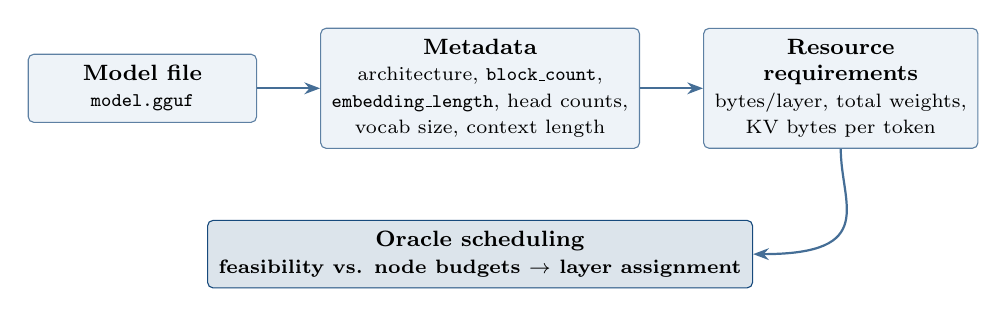
\begin{tikzpicture}[node distance=8mm]
\node[box, minimum width=2.9cm] (m) {\textbf{Model file}\\\scriptsize
  \texttt{model.gguf}};
\node[box, right=of m, minimum width=3.5cm] (meta) {\textbf{Metadata}\\\scriptsize
  architecture, \texttt{block\_count},\\\scriptsize \texttt{embedding\_length},
  head counts,\\\scriptsize vocab size, context length};
\node[box, right=of meta, minimum width=3.3cm] (req) {\textbf{Resource}\\\textbf{requirements}\\\scriptsize
  bytes/layer, total weights,\\\scriptsize KV bytes per token};
\node[dark, below=9mm of meta, minimum width=4.6cm] (sch) {\textbf{Oracle scheduling}\\\scriptsize
  feasibility vs. node budgets $\rightarrow$ layer assignment};
\draw[ar] (m) -- (meta);
\draw[ar] (meta) -- (req);
\draw[ar] (req.south) .. controls +(0,-0.7) and +(1.6,0) .. (sch.east);
\end{tikzpicture}
\caption{From model file to placement decision. Model metadata is read directly
from the file and converted into concrete per-node memory requirements.}
\label{fig:modelrec}
\end{figure}

\begin{itemize}
  \item \textbf{Architecture and layers.} The architecture name and block count
        are read from the file header; the block count directly determines how
        the layer range is divided. \stImp
  \item \textbf{Parameter count and quantisation.} Where the file declares a
        parameter count it is used; otherwise the total is derived from the file
        size on disk, which already reflects the quantisation format. Bytes per
        layer is then total weight bytes divided by layer count. \stImp
  \item \textbf{Memory requirements.} Weight bytes per node follow from bytes per
        layer; KV bytes follow from head counts, head dimension, context length
        and activation data type. Both feed the feasibility check. \stImp
  \item \textbf{Runtime compatibility.} The runner interface abstracts three back
        ends (Accelerate BLAS, Metal, llama.cpp) selected by a command-line flag.
        Automatic selection of the best back end for a given model and host is
        not implemented. \stPlan
\end{itemize}

If no model file is supplied, the geometry falls back to the values in the
cluster configuration file, which lets the placement logic and the transport be
exercised without downloading tens of gigabytes of weights --- a deliberate
convenience during development.

%===================================================== NETWORKING & HEARTBEAT =
\section{Networking and Heartbeat}

\subsection{Physical connectivity}

The reference deployment connects machines over a \textbf{Thunderbolt~3 bridge}
rather than over the office network. The reasons are latency and isolation: a
direct cable between two machines removes switch hops and shared contention from
the inference path, and the cluster's tensor traffic never touches the general
network. The design does not depend on Thunderbolt specifically --- any dedicated
low-latency link, such as a private 10~GbE segment, serves the same role.

\begin{table}[h]
\centering
\caption{Cluster network endpoints in the reference three-node configuration.}
\label{tab:net}
\footnotesize
\begin{tabular}{@{}llll@{}}
\toprule
\textbf{Role} & \textbf{Address} & \textbf{Ports} & \textbf{Traffic} \\
\midrule
Master   & 10.10.0.1 & TCP 8000 / TCP 9200 / UDP 9100 & Client API / tensors / heartbeat \\
Worker 1 & 10.10.0.2 & TCP 9200 / UDP 9100            & Tensors / heartbeat \\
Worker 2 & 10.10.0.3 & TCP 9200 / UDP 9100            & Tensors / heartbeat \\
\bottomrule
\end{tabular}
\end{table}

\subsection{Data transfer and overhead}

Tensors are sent as a packed 76-byte header followed by the raw payload, written
in a single vectored write so that header and body are not copied together first.
\texttt{TCP\_NODELAY} is enabled, because a 16~KiB activation must be sent
immediately rather than waiting for Nagle coalescing. Where two Oracle processes
share a machine, the socket path is replaced by a lock-free shared-memory ring,
removing the kernel round trip entirely.

Communication overhead per generated token is one activation hop per pipeline
stage plus one logits return to the master. This is small in bytes but is paid on
\emph{every} token, so the meaningful metric is round-trip latency, not
bandwidth. The repository ships a dedicated bench tool that measures exactly this
ping-pong; the project's own target gates are $>8$~Gbps of TCP throughput on the
bridge and a decode round trip well under 5~ms. These are design targets, not
results --- see Section~\ref{sec:eval}.

\subsection{Heartbeat and failure detection}

\begin{figure}[h]
\centering
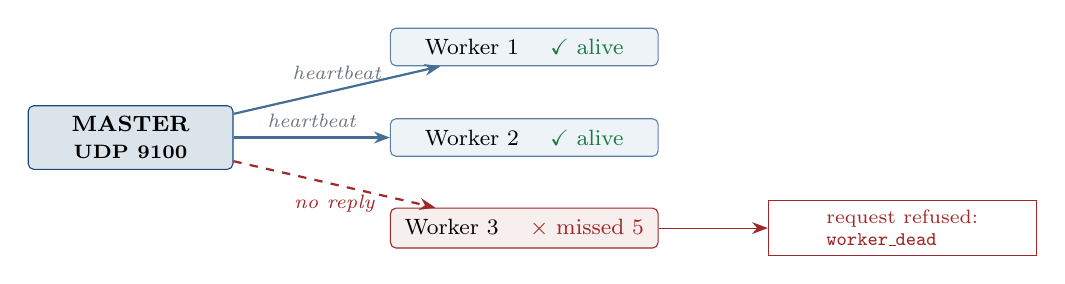
\begin{tikzpicture}
\node[dark, minimum width=2.6cm] (m) at (-4.6,0) {\textbf{MASTER}\\\scriptsize UDP 9100};
\node[box, minimum width=3.4cm] (w1) at (0.4, 1.15)
  {Worker 1 \quad\textcolor{ogreen}{$\checkmark$ alive}};
\node[box, minimum width=3.4cm] (w2) at (0.4, 0.0)
  {Worker 2 \quad\textcolor{ogreen}{$\checkmark$ alive}};
\node[box, minimum width=3.4cm, draw=ored, fill=ored!8] (w3) at (0.4,-1.15)
  {Worker 3 \quad\textcolor{ored}{$\times$ missed 5}};
\draw[ar] (m) -- node[lbl,above]{heartbeat} (w1);
\draw[ar] (m) -- node[lbl,above]{heartbeat} (w2);
\draw[-{Stealth[length=2mm]}, draw=ored, thick, dashed] (m) --
  node[lbl,below,text=ored]{no reply} (w3);
\node[plain, draw=ored, text=ored, align=left, minimum width=3.4cm] (ref) at (5.2,-1.15)
  {request refused:\\\texttt{worker\_dead}};
\draw[arg, draw=ored] (w3) -- (ref);
\end{tikzpicture}
\caption{Heartbeat-based liveness. Each node broadcasts a small datagram every
200~ms; five consecutive missed intervals mark a node dead, and the next request
is refused rather than blocked.}
\label{fig:hb}
\end{figure}

Every node sends a compact UDP datagram carrying the protocol magic number and
its node identifier to each peer at a fixed interval (200~ms by default). Receipt
resets that node's miss counter and refreshes its last-seen timestamp. A periodic
sweep increments the miss counter of any node whose last-seen timestamp is older
than \texttt{interval} $\times$ \texttt{misses}, and marks the node dead once the
threshold (5 by default) is crossed.

The value of this is concrete. Without it, a request routed through a crashed
worker blocks on a socket read until a multi-second timeout expires, and the
client sees a hang. With it, the orchestrator checks liveness \emph{before}
committing to a generation and returns a clear error immediately. The current
prototype detects failure and refuses work; it does \textbf{not} re-shard the
model onto the surviving nodes or retry elsewhere. Automatic recovery is future
work (Section~\ref{sec:future}).

%================================================================== SECURITY ==
\section{Security}

\begin{figure}[h]
\centering
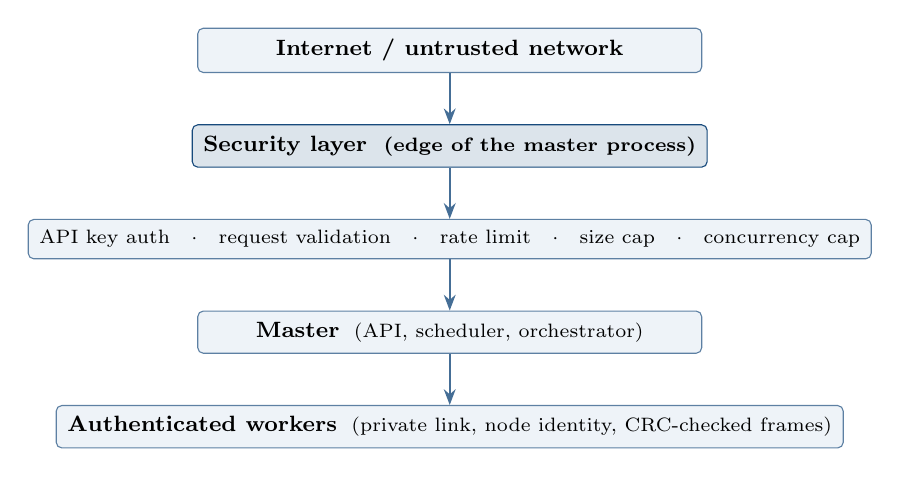
\begin{tikzpicture}[node distance=6.5mm]
\node[box, minimum width=6.4cm] (net) {\textbf{Internet / untrusted network}};
\node[dark, below=of net, minimum width=6.4cm] (sec) {\textbf{Security layer}
  \;\scriptsize(edge of the master process)};
\node[box, below=of sec, minimum width=6.4cm] (ctl)
  {\scriptsize API key auth \; $\cdot$ \; request validation \; $\cdot$ \; rate limit
   \; $\cdot$ \; size cap \; $\cdot$ \; concurrency cap};
\node[box, below=of ctl, minimum width=6.4cm] (mst) {\textbf{Master}
  \;\scriptsize(API, scheduler, orchestrator)};
\node[box, below=of mst, minimum width=6.4cm] (wrk)
  {\textbf{Authenticated workers} \;\scriptsize(private link, node identity,
   CRC-checked frames)};
\draw[ar] (net) -- (sec);
\draw[ar] (sec) -- (ctl);
\draw[ar] (ctl) -- (mst);
\draw[ar] (mst) -- (wrk);
\end{tikzpicture}
\caption{Security architecture. Client-facing controls terminate at the master;
the worker mesh is a separate trust domain reached only over the private link.}
\label{fig:sec}
\end{figure}

Oracle's threat model is modest and stated plainly: the cluster's internal link
is assumed to be physically private, while the master's HTTP port may be exposed
to a wider network. The controls below are grouped by what actually exists.

\begin{table}[h]
\centering
\caption{Security mechanisms and their implementation status.}
\label{tab:sec}
\footnotesize
\begin{tabularx}{\textwidth}{@{}l X l@{}}
\toprule
\textbf{Mechanism} & \textbf{Behaviour} & \textbf{Status} \\
\midrule
Frame integrity & Every tensor frame carries protocol magic, version and a CRC32
  over the payload; malformed or corrupted frames are rejected & \stImp \\
Resource admission & Allocation is refused when it would exceed a node's declared
  budget or overcommit host memory, which bounds memory-exhaustion damage & \stImp \\
Liveness gating & Requests are refused when a required node is unreachable,
  preventing work from being routed into a hole & \stImp \\
Network isolation & Tensor and heartbeat traffic ride a dedicated private link,
  not the general network & \stImp{} (deployment) \\
API authentication & Bearer-token/API-key check on every \texttt{/v1/*} request & \stPlan \\
Request validation & Strict schema validation and bounded field parsing on the
  JSON request body & \stPlan \\
Rate limiting & Per-client request rate ceiling & \stPlan \\
Request-size limits & Maximum body size and maximum \texttt{max\_tokens} & \stPlan \\
Concurrency limits & Cap on simultaneous in-flight generations per client and
  cluster-wide & \stPlan \\
DDoS mitigation & Connection caps, timeouts and early rejection of oversized or
  unauthenticated traffic & \stPlan \\
Worker authentication & Shared-secret or certificate-based node identity so that
  only known workers join the mesh & \stPlan \\
Secure node communication & Encrypted or authenticated tensor channel (currently
  plaintext on a private link) & \stFut \\
Model integrity validation & Checksum verification of model files before load & \stPlan \\
Security event logging & Structured audit log of authentication failures,
  rejections and node state changes & \stPlan \\
\bottomrule
\end{tabularx}
\end{table}

Two limitations deserve emphasis rather than burial. First, the current HTTP
server performs \textbf{no authentication}: anyone who can reach port 8000 can
issue a request, so the prototype must be run on a trusted network or behind a
reverse proxy that supplies these controls. Second, heartbeat datagrams are
\textbf{unauthenticated}, so a host on the internal link could forge liveness for
a node that is actually down. Both are direct consequences of the one-week scope,
and both are addressed by the planned items above. Oracle does not offer
enterprise-grade protection and should not be described as if it did.

%=========================================================== API & INTERFACE ==
\section{API and User Interface}

\subsection{OpenAI-compatible API}

The master exposes an HTTP interface that mirrors the OpenAI chat-completions
protocol on port 8000.

\begin{lstlisting}[language=bash]
GET  /health                 -> {"status":"ok"}
GET  /v1/models              -> list of models served by this cluster
POST /v1/chat/completions    -> chat completion (streaming or buffered)
POST /v1/completions         -> plain completion (same handler)
\end{lstlisting}

\begin{lstlisting}[language=bash]
curl -sS http://10.10.0.1:8000/v1/chat/completions \
  -H 'Content-Type: application/json' \
  -d '{"model":"Oracle",
       "messages":[{"role":"user",
                    "content":"Explain pipeline parallelism."}],
       "max_tokens":128,
       "stream":true}'
\end{lstlisting}

When \texttt{stream} is true the server replies with server-sent events, emitting
one \texttt{chat.\allowbreak completion.\allowbreak chunk} per token as it is produced and terminating
with \texttt{data: [DONE]}, exactly as clients expect.

Compatibility is a deliberate design decision rather than a convenience. Because
the wire format is the one the ecosystem already speaks, existing chat front
ends, SDKs, agent frameworks and simple \texttt{curl} scripts point at Oracle by
changing a base URL and nothing else. The distributed cluster behind the endpoint
is invisible to the client, which is the entire point: complexity stays inside
the platform. The parsing in the current build is a lightweight hand-rolled field
extractor rather than a full JSON parser, and usage accounting is a placeholder ---
both are noted as hardening work.

\subsection{Conceptual dashboard}

The following mock-up shows the operator view Oracle is designed to expose. It is
a \stPlan{} component: no user interface exists in the repository today, and all
values shown are placeholders.

\begin{center}
\setlength{\fboxsep}{7pt}
\fbox{\begin{minipage}{0.80\textwidth}
\ttfamily\footnotesize
\textbf{ORACLE AI PLATFORM}\\[2pt]
\rule{\linewidth}{0.4pt}\\[3pt]
Model:\qquad Qwen / Llama / \ldots\ (80 layers, Q4)\\[4pt]
Cluster:\\
\qquad Master \textcolor{ogreen}{$\bullet$}---- Worker 1 \textcolor{ogreen}{$\bullet$}---- Worker 2 \textcolor{ogreen}{$\bullet$}\\[4pt]
Active requests:\qquad XX\\
Queued requests:\qquad XX\\[4pt]
CPU:\qquad XX\%\qquad RAM:\qquad XX\%\\
GPU:\qquad XX\%\qquad Network:\quad XX Gbps\\[4pt]
Security:\qquad \textcolor{ogreen}{$\checkmark$}\qquad Heartbeat:\quad \textcolor{ogreen}{$\checkmark$}\\
\rule{\linewidth}{0.4pt}
\end{minipage}}
\end{center}

The interface is intended to visualise cluster health (which nodes are alive and
how the layers are distributed), the loaded model and its geometry, request
pressure (active versus queued), per-node resource utilisation, link throughput,
and the state of the security controls --- that is, the same facts the
orchestrator already tracks internally, surfaced for a human operator.

%================================================================ DEPLOYMENT ==
\section{Deployment}

Oracle is deployed as two cooperating processes -- one master, one worker per
additional machine -- driven by a single shared cluster description.

\begin{figure}[h]
\centering
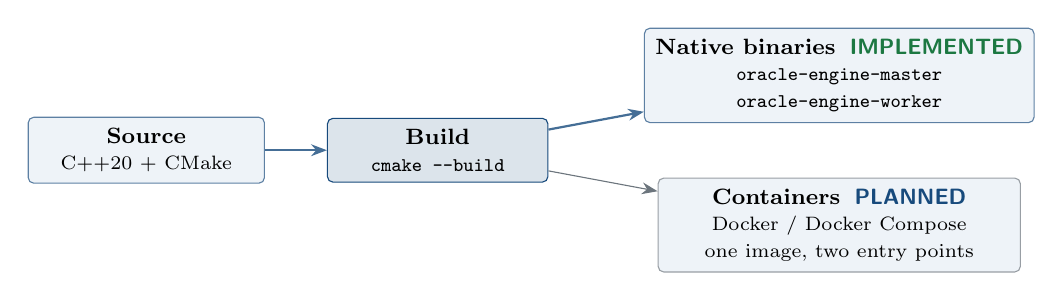
\begin{tikzpicture}
\node[box, minimum width=3.0cm] (src) at (-5.2,0) {\textbf{Source}\\\scriptsize C++20 + CMake};
\node[dark, minimum width=2.8cm] (build) at (-1.5,0) {\textbf{Build}\\\scriptsize
  \texttt{cmake -{}-build}};
\node[box, minimum width=4.6cm] (nat) at (3.6, 0.95)
  {\textbf{Native binaries} \;\stImp\\\scriptsize \texttt{oracle-engine-master}\\
   \scriptsize \texttt{oracle-engine-worker}};
\node[box, minimum width=4.6cm, draw=ogray!70] (ctr) at (3.6,-0.95)
  {\textbf{Containers} \;\stPlan\\\scriptsize Docker / Docker Compose\\
   \scriptsize one image, two entry points};
\draw[ar] (src) -- (build);
\draw[ar] (build) -- (nat);
\draw[arg] (build) -- (ctr);
\end{tikzpicture}
\caption{Deployment paths. Native binaries are the supported route today;
containerisation is designed but not present in the repository.}
\label{fig:deploy}
\end{figure}

\textbf{Native.} The project builds with CMake into three executables:
\texttt{oracle-engine-master} (config, API, cluster bring-up),
\texttt{oracle-engine-worker} (layer execution) and
\texttt{oracle-engine-bench-net} (link measurement), plus an install target that
places them on \texttt{PATH}. All nodes share one \texttt{cluster.toml} that
declares the model, the node list, their addresses and their memory budgets;
each process is told which node it is with \texttt{--id}. A single-machine
smoke mode (\texttt{--single}) collapses the cluster to one node for development.

\begin{lstlisting}[language=bash]
cmake -S . -B build -DORACLE_BUILD_PYTHON=OFF
cmake --build build -j
./build/oracle-engine-master --config configs/cluster.toml --id 0
./build/oracle-engine-worker --config configs/cluster.toml --id 1
\end{lstlisting}

An optional Python extension module exposes the engine for scripting, and a small
Python helper prints the cluster table from the same configuration file.

\textbf{Containerised.} A container image per role, orchestrated with Docker
Compose and sharing a host network so the dedicated link remains visible, is the
intended packaging for reproducible deployment. No Dockerfile exists in the
repository yet; this is \stPlan.

\textbf{Platform note.} The current build targets macOS: the transport uses
\texttt{kqueue}, the CPU back end uses Apple's Accelerate framework, and the GPU
back end uses Metal. Porting the event loop to \texttt{epoll} and the BLAS calls
to a portable library is required for Linux support.

%========================================================= TESTING/EVALUATION =
\section{Testing and Evaluation}
\label{sec:eval}

\subsection{What is tested today}

The repository ships five automated unit tests, run through CTest, covering the
shared-memory ring buffer, the wire protocol encode/decode round trip, the shard
plan (layer coverage, KV sizing, feasibility against budgets), a TCP transport
round trip between two sockets, and a tiny end-to-end pipeline that builds a DAG,
runs a GEMM through both the CPU and GPU back ends, and generates tokens. Four
staged validation scripts cover network benchmarking, allocation dry-run, tensor
pass-through and an end-to-end HTTP smoke test.

\subsection{Evaluation plan}

The metrics below are the ones that matter for a distributed inference platform.
No values are reported, because none have been measured on the target cluster.
Where the project has defined an internal target, it is shown as a gate, not as
a result.

\begin{table}[h]
\centering
\caption{Evaluation metrics, method and current values.}
\label{tab:eval}
\footnotesize
\begin{tabularx}{\textwidth}{@{}l X l l@{}}
\toprule
\textbf{Metric} & \textbf{Method} & \textbf{Target gate} & \textbf{Value} \\
\midrule
Network bandwidth & \texttt{iperf3} + \texttt{oracle-engine-bench-net} over the
  bridge & $>8$ Gbps & \tbm \\
Network latency & Activation-sized ping-pong round trip (16 KiB F16) & $\ll 5$ ms
  & \tbm \\
Model loading time & Wall clock from process start to first ready state & --- & \tbm \\
Inference latency & End-to-end wall clock per request & --- & \tbm \\
Time to first token & Client timestamp of the first SSE chunk & --- & \tbm \\
Throughput (tokens/s) & Tokens generated / elapsed decode time & --- & \tbm \\
Concurrent requests & Maximum sustained in-flight requests without error & --- & \tbm \\
CPU / RAM / GPU utilisation & Per-node sampling during a sustained run & --- & \tbm \\
Worker failure detection & Kill a worker; time until it is marked dead and a
  request is refused & $\le$ interval $\times$ misses & \tbm \\
Request success rate & Successful responses / total requests under load & --- & \tbm \\
\bottomrule
\end{tabularx}
\end{table}

Two of these deserve a note on interpretation. \emph{Time to first token} is
dominated by prefill and by the number of pipeline hops, so it is the metric most
sensitive to adding nodes --- adding a machine buys memory but costs latency.
\emph{Worker failure detection} is directly predictable from configuration
(heartbeat interval $\times$ miss threshold, i.e. one second at the defaults) and
is therefore the easiest end-to-end behaviour to verify experimentally.

%==================================================== LIMITATIONS / FUTURE ====
\section{Limitations, Future Work and Conclusion}
\label{sec:future}

\subsection{Limitations}

\begin{itemize}
  \item \textbf{One-week scope.} The project was built in approximately one week.
        Breadth of the distributed design was prioritised over depth in any single
        component.
  \item \textbf{Model execution is not complete.} The distributed dataflow is
        real; the layer numerics are placeholder. Oracle does not yet produce
        meaningful generated text (Section~5.3).
  \item \textbf{Hardware.} Development targeted a small number of macOS machines
        with modest discrete GPUs. Weights and KV live in system RAM; the GPUs
        act as a small cache, not as the primary compute device.
  \item \textbf{Cluster size.} The design and the configuration have been
        exercised at three nodes. Behaviour at larger scale is untested, and a
        strictly linear pipeline is unlikely to be the right topology beyond a
        handful of nodes.
  \item \textbf{Model coverage.} GGUF metadata parsing targets llama-family
        models. Other architectures and container formats are unhandled.
  \item \textbf{Concurrency.} Per-request isolation inside the engine is
        incomplete, so genuine multi-request serving is not yet demonstrated.
  \item \textbf{Production hardening.} No authentication, no TLS, no rate
        limiting, no automatic recovery, no Linux support, and no measured
        performance figures.
\end{itemize}

\subsection{Future work}

\begin{enumerate}[label=\arabic*.]
  \item \textbf{Real weight execution.} Wire GGUF weight loading and transformer
        kernels into the runner interface so that shards execute genuine layers.
        This unlocks every other measurement in Table~\ref{tab:eval}.
  \item \textbf{Per-request isolation and continuous batching.} Give each
        sequence its own KV slice and pipeline slot, then batch decode steps
        across sequences to raise throughput.
  \item \textbf{Improved KV-cache management.} Paged, block-allocated KV storage
        so that memory is proportional to the tokens actually generated rather
        than to the maximum context length.
  \item \textbf{Automatic model placement.} Weight the layer split by each node's
        measured capability and observed link latency instead of splitting evenly.
  \item \textbf{Smarter scheduling.} Feed live worker load and queue depth into
        placement and admission decisions; a learned policy is a longer-term
        possibility.
  \item \textbf{Automatic failure recovery.} Re-shard onto surviving nodes and
        replay the affected request instead of refusing it.
  \item \textbf{Stronger security.} Implement the planned rows of
        Table~\ref{tab:sec}, starting with API authentication, request limits and
        worker identity.
  \item \textbf{Broader hardware and model support.} Linux (\texttt{epoll},
        portable BLAS, CUDA), and more model architectures.
  \item \textbf{Easier deployment.} Container images, Compose manifests and a
        one-command cluster bring-up, plus the operator dashboard.
\end{enumerate}

\subsection{Conclusion}

Oracle demonstrates the concept of turning multiple physically connected
computers into a coordinated AI inference platform capable of distributing large
AI workloads while supporting concurrent requests, orchestration, monitoring, and
security. Within a one-week scope the project delivers the parts that are
genuinely hard to retrofit: a compact binary tensor protocol with integrity
checking, a memory-aware sharding planner that refuses infeasible clusters before
they fail, a pipeline orchestrator that traverses a multi-machine layer graph,
heartbeat-based liveness that turns a hang into a clear error, and a standard
OpenAI-compatible endpoint that hides all of it from the client.

What remains is equally clear, and this report has been explicit about it:
executing real model weights, isolating concurrent requests, and implementing the
security layer. Those are additions to a working skeleton rather than a change of
direction --- which is the most useful thing a one-week prototype can establish.

%=============================================================== REFERENCES ===
\begin{thebibliography}{9}
\footnotesize
\bibitem{vaswani} A.~Vaswani et al., ``Attention Is All You Need,''
  \emph{NeurIPS}, 2017.
\bibitem{gpipe} Y.~Huang et al., ``GPipe: Efficient Training of Giant Neural
  Networks using Pipeline Parallelism,'' \emph{NeurIPS}, 2019.
\bibitem{megatron} M.~Shoeybi et al., ``Megatron-LM: Training Multi-Billion
  Parameter Language Models Using Model Parallelism,'' arXiv:1909.08053, 2019.
\bibitem{vllm} W.~Kwon et al., ``Efficient Memory Management for Large Language
  Model Serving with PagedAttention,'' \emph{SOSP}, 2023.
\bibitem{orca} G.-I.~Yu et al., ``Orca: A Distributed Serving System for
  Transformer-Based Generative Models,'' \emph{OSDI}, 2022.
\bibitem{petals} A.~Borzunov et al., ``Petals: Collaborative Inference and
  Fine-tuning of Large Models,'' arXiv:2209.01188, 2022.
\bibitem{llamacpp} G.~Gerganov et al., ``llama.cpp and the GGUF model format,''
  \url{https://github.com/ggml-org/llama.cpp}.
\bibitem{httplib} Y.~Hirose, ``cpp-httplib: a C++11 single-file header-only HTTP
  library,'' \url{https://github.com/yhirose/cpp-httplib}.
\bibitem{openai} OpenAI, ``API Reference: Chat Completions,''
  \url{https://platform.openai.com/docs/api-reference/chat}.
\end{thebibliography}

\end{document}
